%%%%%%%%%%%%%%%%%%%%%%%%%%%%%%%%%%%%%%%%%%%%%%%%%%%%%%%%
%%
\clearpage
\newpage
\section{The cal\_loc recipe}
\label{ch:the_recipes:cal_loc_RAW_spirou}
%%
%%%%%%%%%%%%%%%%%%%%%%%%%%%%%%%%%%%%%%%%%%%%%%%%%%%%%%%%

Locates the orders on the `dark\_flat' or `flat\_dark' images.\\

% -------------------------------------------------------
\subsection{The inputs}
% -------------------------------------------------------
The input of \callocRAW is as follows:
\begin{cmdbox}
cal_loc_RAW_spirou.py night_repository filenames
\end{cmdbox}
\noindent for example:
\begin{cmdbox}[title={example}]
cal_loc_RAW_spirou.py 20170710 flat_dark02f10.fits
\end{cmdbox}
\noindent or
\begin{pythonbox}
import cal_loc_RAW_spirou
night_repository = '20170710'
filenames = ['flat_dark02f10.fits']
cal_loc_RAW_spirou.main(night_repository, files=filenames)
\end{pythonbox}

\noindent where `night\_repository' defines \argnightname and `filenames' define the list of files in \argfilenames. All files in filenames must be valid python strings separated by a space (command line) or in a line (python) and must have the folowing prefixes:
\noindent File prefixes allowed:
\begin{itemize}
	\item dark\_flat
	\item flat\_dark
\end{itemize}

% -------------------------------------------------------
\subsection{The outputs}
% -------------------------------------------------------
The outputs of \callocRAW are as follows:

\begin{itemize}
\item \definevariable{text:order_profile}{order\_profile} in form:
\begin{tcustomdir}
\{\reduceddir\}/\{date prefix\}\_\{file\}\_order\_profile\_\{fiber\}.fits
\end{tcustomdir}

\item \definevariable{text:locofitsfile}{locofitsfile} in form:
\begin{tcustomdir}
\{\reduceddir\}/\{date prefix\}\_\{file\}\_loco\_\{fiber\}.fits
\end{tcustomdir}

\item \definevariable{text:locofitsfile2}{locofitsfile2} in form:
\begin{tcustomdir}
\{\reduceddir\}/\{date prefix\}\_\{file\}\_fwhm-order\_\{fiber\}.fits
\end{tcustomdir}

\item \definevariable{text:locofitsfile3}{locofitsfile3} in form:
\begin{tcustomdir}
\{\reduceddir\}/\{date prefix\}\_\{file\}\_with-order\_\{fiber\}.fits
\end{tcustomdir}

\end{itemize}

\noindent where `date prefix' is constructed from \argnightname and the file name is the first file in \argfilenames. \\

\clearpage
\newpage

\noindent For example for \reduceddir\lstinline[style=pythoninline]|='/drs/data/reduced/20170710'| and \argfilenames\lstinline[style=pythoninline]|=['flat_dark02f10.fits']| the output files would be:
\begin{tcustomdir}
\begin{itemize}
\item /drs/data/reduced/20170710/20170710\_flat\_dark02f10\_order\_profile\_\{fiber\}.fits
\item /drs/data/reduced/20170710/20170710\_flat\_dark02f10\_loco\_\{fiber\}.fits
\item /drs/data/reduced/20170710/20170710\_flat\_dark02f10\_fwhm-order\_\{fiber\}.fits
\item /drs/data/reduced/20170710/20170710\_flat\_dark02f10\_with-order\_\{fiber\}.fits
\end{itemize}
\end{tcustomdir}

% -------------------------------------------------------
\subsection{Summary of procedure}
% -------------------------------------------------------
\begin{enumerate}
\item adds all defined `dark\_flat' or `flat\_dark' files together
\item corrects for darks
\item resizes the image
\item constructs `order\_profile' image
\item locates the central pixel of each order
\item steps out in large steps along the order (toward beginning and end)
\item fits the position of each order (using a small 2D box around each fit point)
	\begin{itemize}
	\item includes a rejection of bad points (while loop)
	\end{itemize}
\item fits the width of each order (using a small 2D box around each fit point)
	\begin{itemize}
	\item includes a rejection of bad points (while loop)
	\end{itemize}
\item saves the `order\_profile' image (with a superposition of the fit orders as zero values)
\item does some quality control
\item updates calibDB with key ``LOC\_{fiber}'' where {fiber} = [AB, C] etc
\end{enumerate}



% -------------------------------------------------------
\subsection{Quality Control}
% -------------------------------------------------------

There are currently five quality control checks for \callocRAW
\begin{itemize}

\item Too many rejected orders in center position fit: 
	\begin{thighlight}
	\begin{equation}
	\text{Number of rejected orders in center fit} > \text{\definevariable{text:qc_loc_maxlocfit_removed_ctr}{\path{qc_loc_maxlocfit_removed_ctr}}}
	\end{equation}
	\end{thighlight}

\item Too many rejected orders in width fit:
	\begin{thighlight}
	\begin{equation}
	\text{Number of rejected orders in width fit} > \text{\definevariable{text:qc_loc_maxlocfit_removed_wid}{\path{qc_loc_maxlocfit_removed_wid}}}
	\end{equation}
	\end{thighlight}

\item RMS on center fit too high: 
	\begin{thighlight}
	\begin{equation}
	\text{Mean rms center fit} > \text{\definevariable{text:qc_loc_rmsmax_center}{\path{qc_loc_rmsmax_center}}}
	\end{equation}
	\end{thighlight}

\item RMS on width fit too high: 
	\begin{thighlight}
	\begin{equation}
	\text{Mean rms width fit} > \text{\definevariable{text:qc_loc_rmsmax_fwhm}{\path{qc_loc_rmsmax_fwhm}}}
	\end{equation}
	\end{thighlight}

\item Abnormal number of identified orders: 
	\begin{thighlight}
	\begin{equation}
	\text{Number of orders found} \neq \text{\definevariable{text:qc_loc_nbo_fpall}{\path{qc_loc_nbo}}}
	\end{equation}
	\end{thighlight}

\end{itemize}

\noindent If none of these quality control criteria are valid then the output file is passed into the \calibdb with key `LOC\_\{fiber\}' for the `locofitsname' file. \\

\noindent For example the following lines are added to the \calibdb for 
\argnightname{\lstinline[style=pythoninline]| = "20170710" |} and \argfilenames{\lstinline[style=pythoninline]| = ["flat_dark02f10.fits"] |}. \\

\begin{textbox}[title={In calibration database file}]
LOC_AB 20170710 20170710_flat_dark02f10_loco_AB.fits 2017-07-10-13:07:08.460000 1499692028.46
\end{textbox}


% -------------------------------------------------------
\subsection{Example working run}
% -------------------------------------------------------

An example run where everything worked is below:

\begin{cmdbox}[title={example}]
cal_loc_RAW_spirou.py 20170710 flat_dark02f10.fits
\end{cmdbox}
\begin{cmdboxprintspecial}[fontupper=\tiny, fontlower=\tiny]
@gHH:MM:SS.S -   || *****************************************@g
@gHH:MM:SS.S -   || * SPIROU \@(#) Geneva Observatory (0.1.015)@g
@gHH:MM:SS.S -   || *****************************************@g
@gHH:MM:SS.S -   ||(dir_data_raw)      DRS_DATA_RAW=/drs/data/raw@g
@gHH:MM:SS.S -   ||(dir_data_reduc)    DRS_DATA_REDUC=/drs/data/reduced@g
@gHH:MM:SS.S -   ||(dir_calib_db)      DRS_CALIB_DB=/drs/data/calibDB@g
@gHH:MM:SS.S -   ||(dir_data_msg)      DRS_DATA_MSG=/drs/data/msg@g
@gHH:MM:SS.S -   ||(print_level)       PRINT_LEVEL=all         %(error/warning/info/all)@g
@gHH:MM:SS.S -   ||(log_level)         LOG_LEVEL=all         %(error/warning/info/all)@g
@gHH:MM:SS.S -   ||(plot_graph)        DRS_PLOT=1            %(def/undef/trigger)@g
@gHH:MM:SS.S -   ||(used_date)         DRS_USED_DATE=undefined@g
@gHH:MM:SS.S -   ||(working_dir)       DRS_DATA_WORKING=/drs/data/tmp@g
@gHH:MM:SS.S -   ||                    DRS_INTERACTIVE is not set, running on-line mode@g
@gHH:MM:SS.S -   ||                    DRS_DEBUG is set, debug mode level:1@g
@gHH:MM:SS.S -   |cal_loc_RAW_spirou:02f10|Now running : cal_loc_RAW_spirou on file(s): flat_dark02f10.fits@g
@gHH:MM:SS.S -   |cal_loc_RAW_spirou:02f10|On directory /drs/data/raw/20170710@g
@gHH:MM:SS.S -   |cal_loc_RAW_spirou:02f10|ICDP_NAME loaded from: /drs/spirou_py3/INTROOT/config/constants_SPIROU.py@g
@gHH:MM:SS.S - * |cal_loc_RAW_spirou:02f10|Correct type of image for localisation (dark_flat or flat_dark)@g
@gHH:MM:SS.S -   |cal_loc_RAW_spirou:02f10|Calibration file: 20170710_flat_flat02f10_badpixel.fits already exists - not copied@g
@gHH:MM:SS.S -   |cal_loc_RAW_spirou:02f10|Calibration file: 20170710_dark_dark02d406.fits already exists - not copied@g
...
@gHH:MM:SS.S - * |cal_loc_RAW_spirou:02f10|Now processing Image TYPE UNKNOWN with cal_loc_RAW_spirou recipe@g
@gHH:MM:SS.S -   |cal_loc_RAW_spirou:02f10|Reading Image /drs/data/raw/20170710/flat_dark02f10.fits@g
@gHH:MM:SS.S -   |cal_loc_RAW_spirou:02f10|Image 2048 x 2048 loaded@g
@gHH:MM:SS.S -   |cal_loc_RAW_spirou:02f10|Doing Dark Correction using /drs/data/calibDB/20170710_dark_dark02d406.fits@g
@gHH:MM:SS.S -   |cal_loc_RAW_spirou:02f10|Image format changed to 1930x2035@g
@gHH:MM:SS.S -   |cal_loc_RAW_spirou:02f10|Saving processed raw frame in 20170710_flat_dark02f10_order_profile_AB.fits
@g@yHH:MM:SS.S - \@ |python warning Line 980  warning reads: Card is too long, comment will be truncated.|@y@g@g
@gHH:MM:SS.S - * |cal_loc_RAW_spirou:02f10|Updating Calib Data Base with ORDER_PROFILE_AB@g
@gHH:MM:SS.S - * |cal_loc_RAW_spirou:02f10|Maximum flux/pixel in the spectrum: 82388.4 [e-]@g
@gHH:MM:SS.S - * |cal_loc_RAW_spirou:02f10|Average background level: 1.39 [%]@g
@gHH:MM:SS.S -   |cal_loc_RAW_spirou:02f10|Searching order center on central column@g
@gHH:MM:SS.S - * |cal_loc_RAW_spirou:02f10|On fiber AB 36 orders have been detected on 2 fiber(s)@g
@gHH:MM:SS.S -   |cal_loc_RAW_spirou:02f10|ORDER: 0 center at pixel 102.5 width 11.6 rms 0.049@g
@gHH:MM:SS.S -   |cal_loc_RAW_spirou:02f10| - center fit rms/ptp/sigrms: 0.049/0.140/2.855 with 0 rejected points@g
@gHH:MM:SS.S -   |cal_loc_RAW_spirou:02f10| - width  fit rms/ptp/ptp%: 0.434/0.740/6.726 with 0 rejected points@g
@gHH:MM:SS.S -   |cal_loc_RAW_spirou:02f10|ORDER: 1 center at pixel 116.9 width 11.4 rms 0.073@g
@gHH:MM:SS.S -   |cal_loc_RAW_spirou:02f10| - center fit rms/ptp/sigrms: 0.073/0.164/2.240 with 0 rejected points@g
@gHH:MM:SS.S -   |cal_loc_RAW_spirou:02f10| - width  fit rms/ptp/ptp%: 0.448/0.794/6.618 with 0 rejected points@g
@gHH:MM:SS.S -   |cal_loc_RAW_spirou:02f10|ORDER: 2 center at pixel 149.8 width 11.7 rms 0.049@g
@gHH:MM:SS.S -   |cal_loc_RAW_spirou:02f10| - center fit rms/ptp/sigrms: 0.049/0.116/2.374 with 0 rejected points@g
@gHH:MM:SS.S -   |cal_loc_RAW_spirou:02f10| - width  fit rms/ptp/ptp%: 0.421/0.881/8.006 with 0 rejected points@g
@gHH:MM:SS.S -   |cal_loc_RAW_spirou:02f10|ORDER: 3 center at pixel 164.2 width 11.5 rms 0.075@g
@gHH:MM:SS.S -   |cal_loc_RAW_spirou:02f10| - center fit rms/ptp/sigrms: 0.075/0.173/2.309 with 0 rejected points@g
@gHH:MM:SS.S -   |cal_loc_RAW_spirou:02f10| - width  fit rms/ptp/ptp%: 0.420/0.806/7.119 with 0 rejected points@g
@gHH:MM:SS.S -   |cal_loc_RAW_spirou:02f10|ORDER: 4 center at pixel 196.6 width 11.5 rms 0.051@g
@gHH:MM:SS.S -   |cal_loc_RAW_spirou:02f10| - center fit rms/ptp/sigrms: 0.051/0.140/2.762 with 0 rejected points@g
@gHH:MM:SS.S -   |cal_loc_RAW_spirou:02f10| - width  fit rms/ptp/ptp%: 0.403/0.989/8.889 with 0 rejected points@g
...
@gHH:MM:SS.S -   |cal_loc_RAW_spirou:02f10|ORDER: 69 center at pixel 1801.4 width 10.4 rms 0.168@g
@gHH:MM:SS.S -   |cal_loc_RAW_spirou:02f10|      center fit converging with rms/ptp/sigrms: 0.168/1.465/8.710@g
@gHH:MM:SS.S -   |cal_loc_RAW_spirou:02f10| - center fit rms/ptp/sigrms: 0.067/0.167/2.490 with 1 rejected points@g
@gHH:MM:SS.S -   |cal_loc_RAW_spirou:02f10|      fwhm fit converging with rms/ptp/ptp%: 0.535/2.337/29.218@g
@gHH:MM:SS.S -   |cal_loc_RAW_spirou:02f10|      fwhm fit converging with rms/ptp/ptp%: 0.478/1.105/11.053@g
@gHH:MM:SS.S -   |cal_loc_RAW_spirou:02f10| - width  fit rms/ptp/ptp%: 0.466/0.936/9.357 with 2 rejected points@g
@gHH:MM:SS.S -   |cal_loc_RAW_spirou:02f10|ORDER: 70 center at pixel 1851.8 width 7.1 rms 2.565@g
@gHH:MM:SS.S -   |cal_loc_RAW_spirou:02f10|      center fit converging with rms/ptp/sigrms: 2.565/8.719/3.399@g
@gHH:MM:SS.S -   |cal_loc_RAW_spirou:02f10| - center fit rms/ptp/sigrms: 0.077/0.158/2.047 with 22 rejected points@g
@gHH:MM:SS.S -   |cal_loc_RAW_spirou:02f10|      fwhm fit converging with rms/ptp/ptp%: 1.070/2.674/44.574@g
...
@gHH:MM:SS.S -   |cal_loc_RAW_spirou:02f10| - width  fit rms/ptp/ptp%: 0.300/0.623/9.965 with 17 rejected points@g
@gHH:MM:SS.S -   |cal_loc_RAW_spirou:02f10|ORDER: 71 center at pixel 1869.1 width 10.7 rms 0.296@g
@gHH:MM:SS.S -   |cal_loc_RAW_spirou:02f10|      center fit converging with rms/ptp/sigrms: 0.296/0.889/3.008@g
...
@gHH:MM:SS.S -   |cal_loc_RAW_spirou:02f10| - center fit rms/ptp/sigrms: 0.099/0.199/1.998 with 30 rejected points@g
@gHH:MM:SS.S -   |cal_loc_RAW_spirou:02f10|      fwhm fit converging with rms/ptp/ptp%: 0.995/3.544/23.627@g
...
@gHH:MM:SS.S -   |cal_loc_RAW_spirou:02f10| - width  fit rms/ptp/ptp%: 0.468/0.838/8.383 with 23 rejected points@g
@gHH:MM:SS.S - * |cal_loc_RAW_spirou:02f10|On fiber AB 72 orders geometry have been measured@g
@gHH:MM:SS.S - * |cal_loc_RAW_spirou:02f10|Average uncertainty on position: 66.42 [mpix]@g
@gHH:MM:SS.S - * |cal_loc_RAW_spirou:02f10|Average uncertainty on width: 381.93 [mpix]@g
@gHH:MM:SS.S - * |cal_loc_RAW_spirou:02f10|QUALITY CONTROL SUCCESSFUL - Well Done -@g
@gHH:MM:SS.S -   |cal_loc_RAW_spirou:02f10|Saving localization information in file: 20170710_flat_dark02f10_loco_AB.fits
@g@yHH:MM:SS.S - \@ |python warning Line 980  warning reads: Card is too long, comment will be truncated.| @y@g@g
@gHH:MM:SS.S -   |cal_loc_RAW_spirou:02f10|Saving FWHM information in file: 20170710_flat_dark02f10_fwhm-order_AB.fits
@g@yHH:MM:SS.S - \@ |python warning Line 980  warning reads: Card is too long, comment will be truncated.|@y@g@g
@gHH:MM:SS.S -   |cal_loc_RAW_spirou:02f10|Saving localization image with superposition of orders in@g
@gHH:MM:SS.S -   |cal_loc_RAW_spirou:02f10|file: 20170710_flat_dark02f10_with-order_AB.fits@g
@gHH:MM:SS.S - * |cal_loc_RAW_spirou:02f10|Updating Calib Data Base with LOC_AB@g
@gHH:MM:SS.S - * |cal_loc_RAW_spirou:02f10|Recipe cal_loc_RAW_spirou has been successfully completed@g
\end{cmdboxprintspecial}


% % -------------------------------------------------------
% \newpage
% \subsection{Interactive mode}
% % -------------------------------------------------------

% \noindent In interactive mode three figures will also appear (see Figure \ref{figure:}).

% \begin{figure}

% \begin{center}
% \begin{minipage}{.495\textwidth}
% \begin{center}
% \includegraphics[width=\textwidth]{Figures/cal_DARK_spirou_1.pdf}
% a
% \end{center}
% \end{minipage}%
% \begin{minipage}{.495\textwidth}
% \begin{center}
% \includegraphics[width=\textwidth]{Figures/cal_DARK_spirou_2.pdf}
% b
% \end{center}
% \end{minipage}%
% \end{center}

% \begin{center}
% \begin{minipage}{.495\textwidth}
% \begin{center}
% \includegraphics[width=\textwidth]{Figures/cal_DARK_spirou_3.pdf}
% c
% \end{center}
% \end{minipage}%
% \end{center}

% \caption{\textbf{(a)} The image with overplot red and blue regions (red/blue rectangles). \textbf{(b)} The bad pixel mask, bad pixels have a value=1 (in black) and good pixels have a value=0 (in white). \textbf{(c)} Histograms of the image regions, the full image (in green), the blue section (in blue) and the red section (in red). \label{figure:cal_DARK_spirou}}
% \end{figure}
